\documentclass[12pt, a4]{article}
\usepackage[english]{babel}
\usepackage[utf8x]{inputenc}
\usepackage{fullpage}
\usepackage{listings}
\usepackage{graphicx}
\usepackage{color}

%Syntax highlighting
\definecolor{blue-violet}{rgb}{0.54, 0.17, 0.89}
\definecolor{ao}{rgb}{0.0, 0.5, 0.0}
\definecolor{amaranth}{rgb}{0.9, 0.17, 0.31}
\definecolor{ballblue}{rgb}{0.13, 0.67, 0.8}
\definecolor{onyx}{rgb}{0.06, 0.06, 0.06}


\lstset{
  breaklines=true,                 % automatic line breaking only at whitespace
  captionpos=b,                    % sets the caption-position to bottom
  breakatwhitespace=false,
  keepspaces=true,
  numbers=left,
  numbersep=5pt,
  showspaces=false,
  showstringspaces=false,
  showtabs=false,
  tabsize=4,  
  backgroundcolor=\color{white},   % choose the background color
  commentstyle=\color{ao},    % comment style
  keywordstyle=\color{amaranth},    % keyword style
  stringstyle=\color{blue-violet},    % string literal style
  numberstyle=\tiny\color{ballblue},	   % number style
  basicstyle=\ttfamily\footnotesize\color{onyx} % size of fonts used for the code
}

%Document Header
\title{\textbf{Department of CSE\\SSN College of Engineering}}
\author{\textbf{Vishakan Subramanian - 18 5001 196 - Semester VII}}
\date{25 August 2021}

\begin{document}
\maketitle
\hrule
\section*{\center{UCS 1712 - Graphics And Multimedia Lab}}
\hrule
\bigskip

%Assignment Details
\subsection*{\center{\textbf{Exercise 5: 2D Transformations in C++ using OpenGL}}}
\subsection*{\flushleft{Aim:}}
\begin{flushleft}

To apply the following 2D transformations on objects and to render the final output along with the
original object.

\begin{itemize}
\item Translation
\item Rotation
	\begin{itemize}
		\item About Origin
		\item With Respect to a fixed point $(x_r, y_r)$
	\end{itemize}
\item Scaling with respect to
	\begin{itemize}
		\item Origin - Uniform vs. Differential Scaling
		\item Fixed Point $(x_f, y_f)$
	\end{itemize}
\newpage
\item Reflection with respect to
	\begin{itemize}
		\item X - Axis
		\item Y - Axis
		\item Origin
		\item The Line $X = Y$
	\end{itemize}
\item Shearing
	\begin{itemize}
		\item X - Direction Shear
		\item Y - Direction Shear
	\end{itemize}
\end{itemize}


\textbf{Note}: Use Homogeneous coordinate representations and matrix multiplication to perform transformations. Divide the output window into four quadrants. 
\newline (Use LINES primitive to draw X \& Y Axes)
 
\end{flushleft}

%Code
\newpage
\subsection*{\flushleft{Code: 2D Transformations:}}
\begin{flushleft}
\lstinputlisting[language = C++]{Transformations/main.cpp}
\end{flushleft}


%Output
\newpage
\subsection*{\flushleft{Output: Initial Plot With Transformations Menu}}
\begin{figure}[h]
\centering
\caption{Initial Plot With Transformations Menu.}
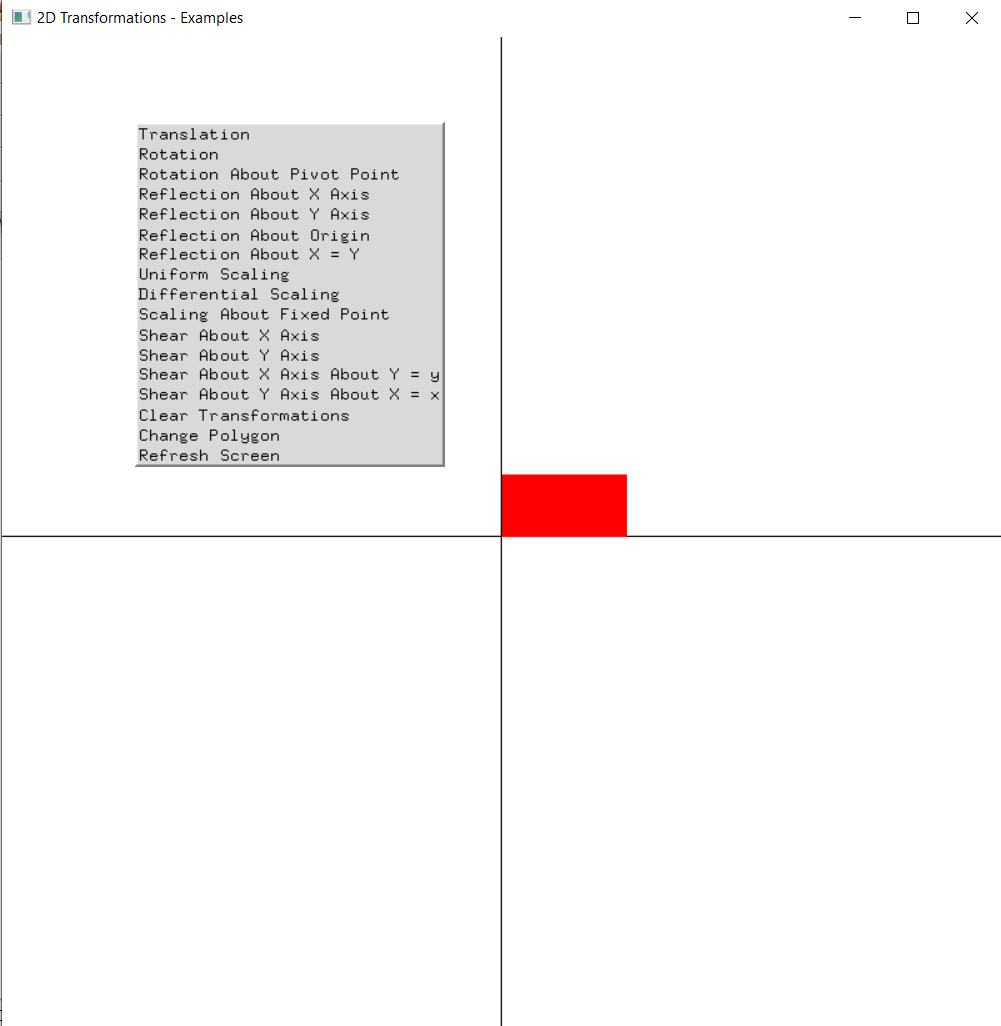
\includegraphics[height=15cm, width=15cm]{Outputs/Output-1.png}
\end{figure}

%Output
\newpage
\subsection*{\flushleft{Output: Console}}
\begin{figure}[h]
\centering
\caption{Output: Console.}
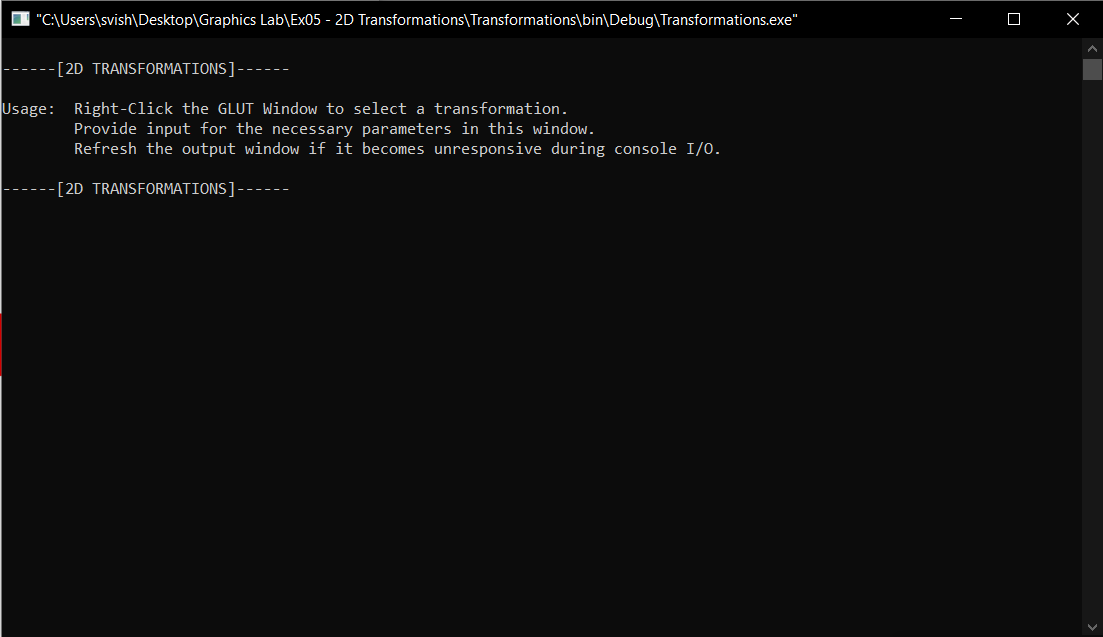
\includegraphics[height=12cm, width=17cm]{Outputs/Console-1.png}
\end{figure}

%Output
\newpage
\subsection*{\flushleft{Output: Translation}}
\begin{figure}[h]
\centering
\caption{Translation by $(10, 20)$.}
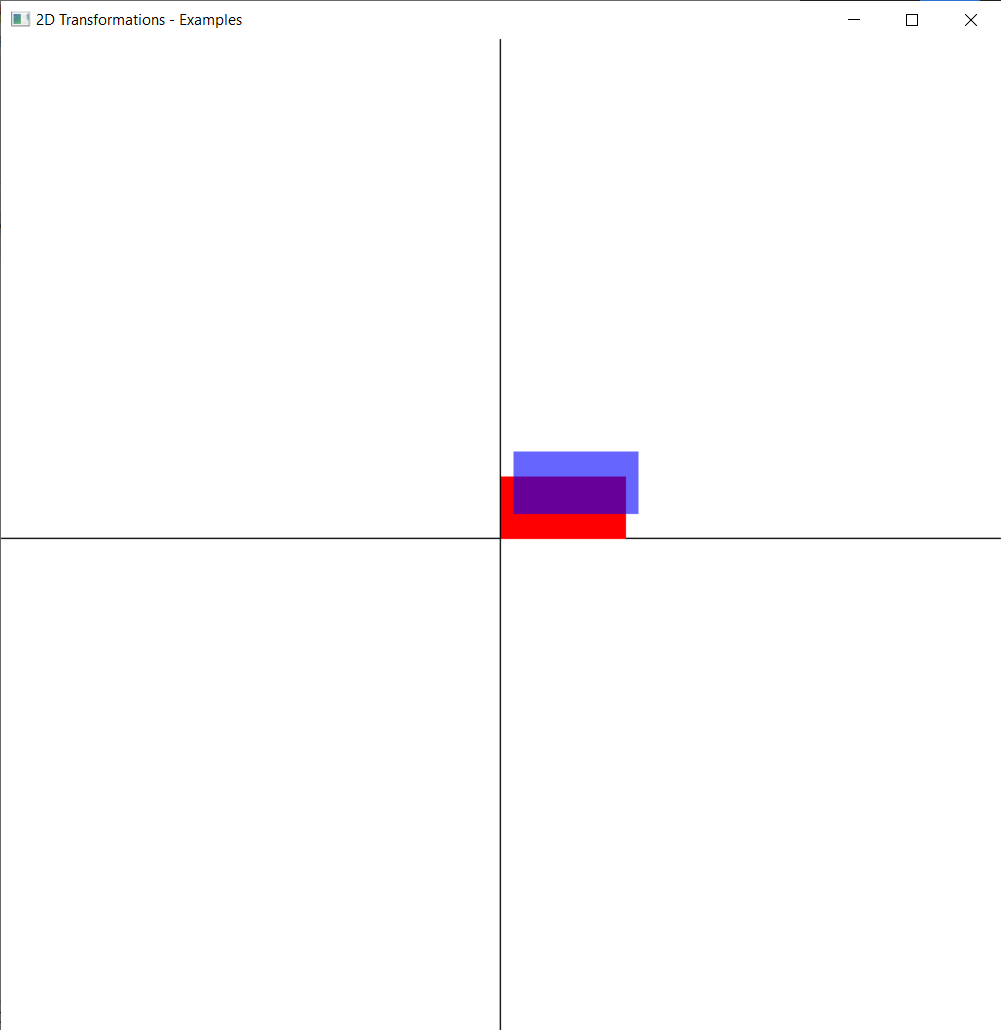
\includegraphics[height=15cm, width=15cm]{Outputs/Output-2.png}
\end{figure}

%Output
\newpage
\subsection*{\flushleft{Output: Rotation}}
\begin{figure}[h]
\centering
\caption{Rotation by $120^{\circ}$.}
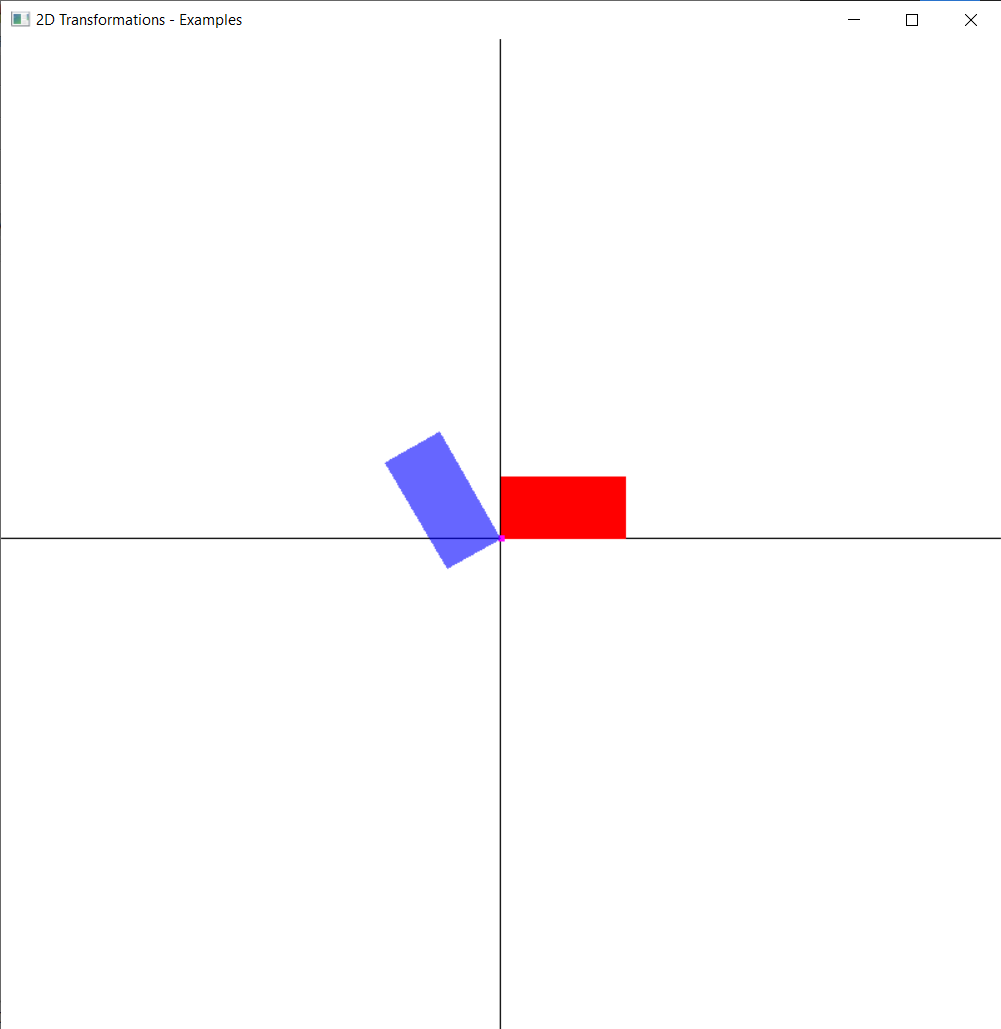
\includegraphics[height=15cm, width=15cm]{Outputs/Output-3.png}
\end{figure}

%Output
\newpage
\subsection*{\flushleft{Output: Rotation About A Pivot Point}}
\begin{figure}[h]
\centering
\caption{Rotation About A Pivot Point $(-50, -50)$ by $90^{\circ}$.}
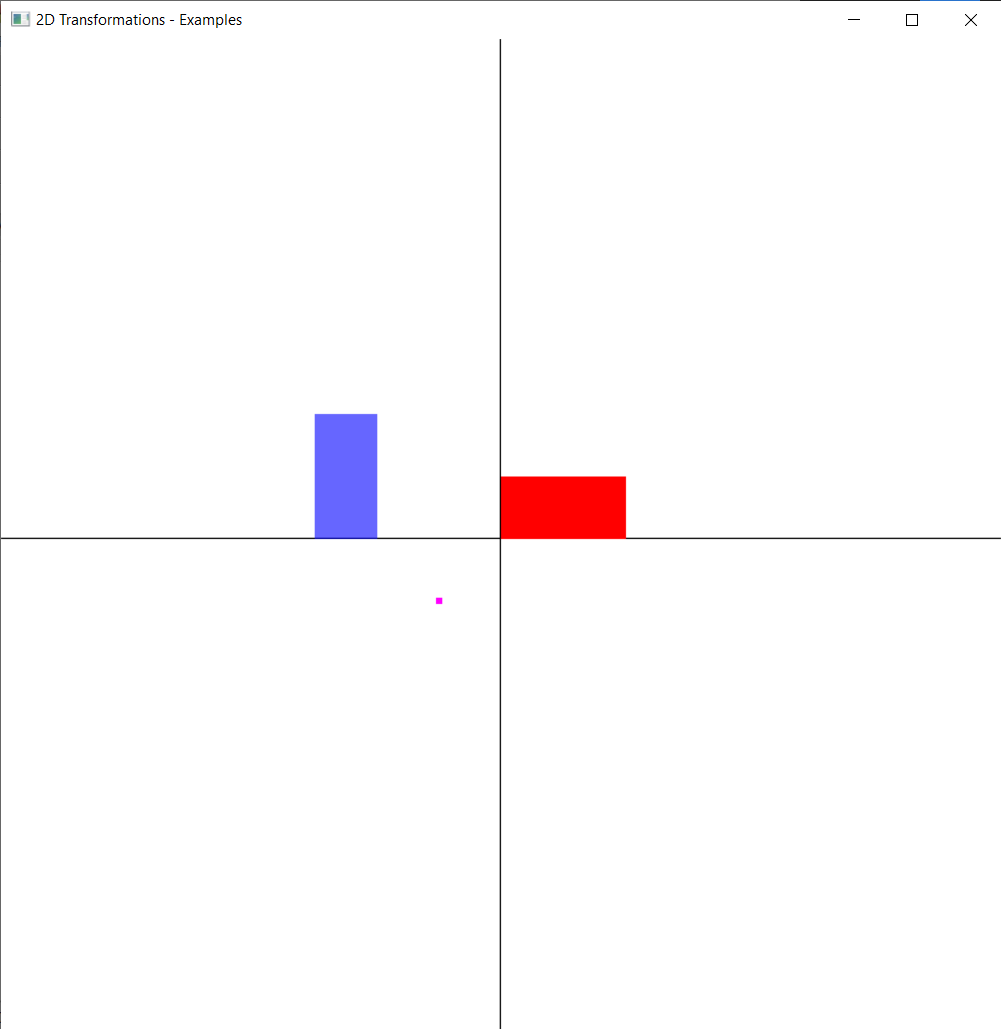
\includegraphics[height=15cm, width=15cm]{Outputs/Output-4.png}
\end{figure}

%Output
\newpage
\subsection*{\flushleft{Output: Console}}
\begin{figure}[h]
\centering
\caption{Console.}
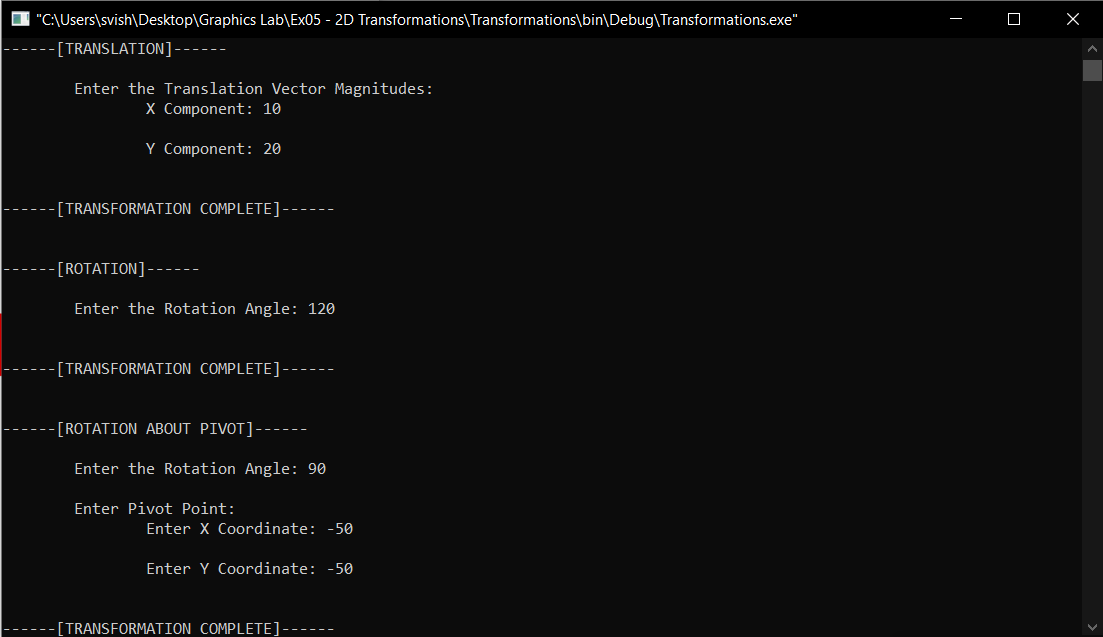
\includegraphics[height=12cm, width=17cm]{Outputs/Console-4.png}
\end{figure}

%Output
\newpage
\subsection*{\flushleft{Output: Reflection About X Axis}}
\begin{figure}[h]
\centering
\caption{Reflection About X Axis.}
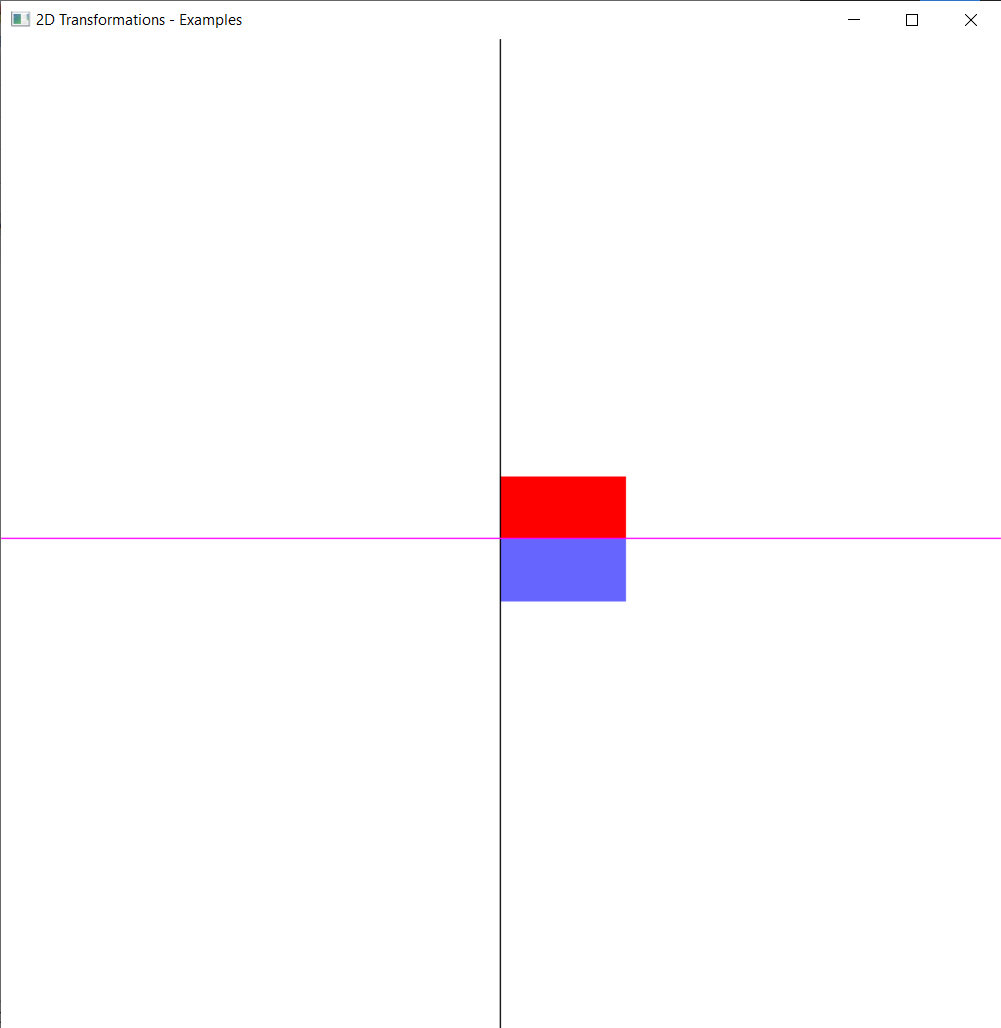
\includegraphics[height=15cm, width=15cm]{Outputs/Output-5.png}
\end{figure}

%Output
\newpage
\subsection*{\flushleft{Output: Reflection About Y Axis}}
\begin{figure}[h]
\centering
\caption{Reflection About Y Axis.}
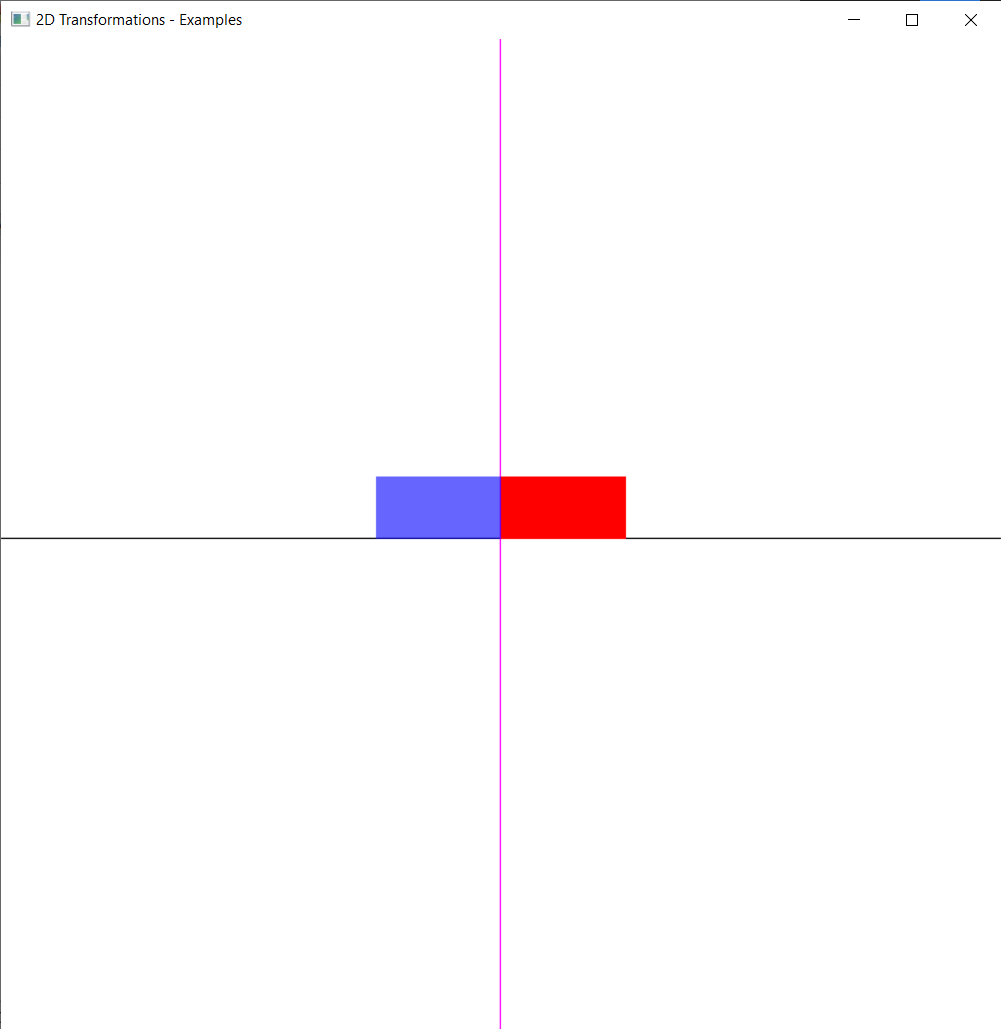
\includegraphics[height=15cm, width=15cm]{Outputs/Output-6.png}
\end{figure}

%Output
\newpage
\subsection*{\flushleft{Output: Reflection About Origin}}
\begin{figure}[h]
\centering
\caption{Reflection About Origin.}
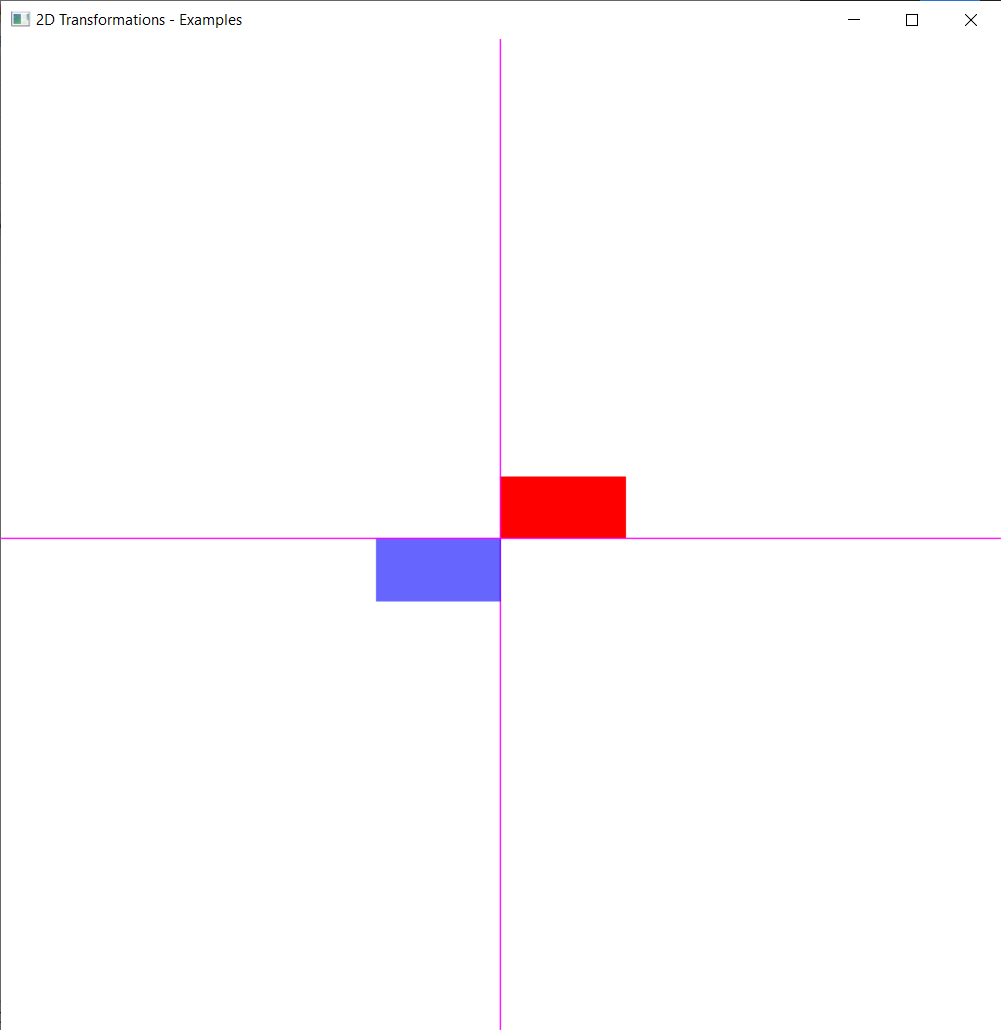
\includegraphics[height=15cm, width=15cm]{Outputs/Output-7.png}
\end{figure}

%Output
\newpage
\subsection*{\flushleft{Output: Reflection About Line $X = Y$}}
\begin{figure}[h]
\centering
\caption{Reflection About Line $X = Y$.}
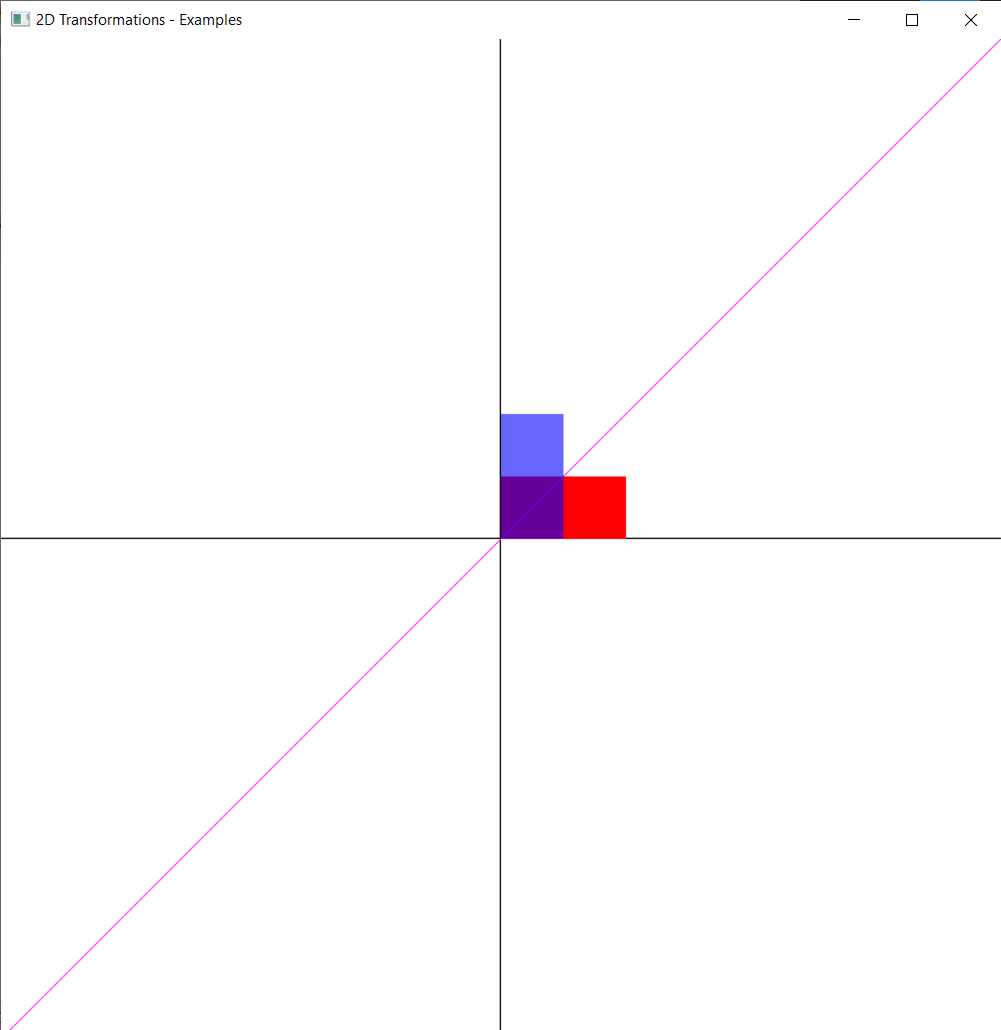
\includegraphics[height=15cm, width=15cm]{Outputs/Output-8.png}
\end{figure}

%Output
\newpage
\subsection*{\flushleft{Output: Uniform Scaling}}
\begin{figure}[h]
\centering
\caption{Uniform Scaling by a Factor of 2.}
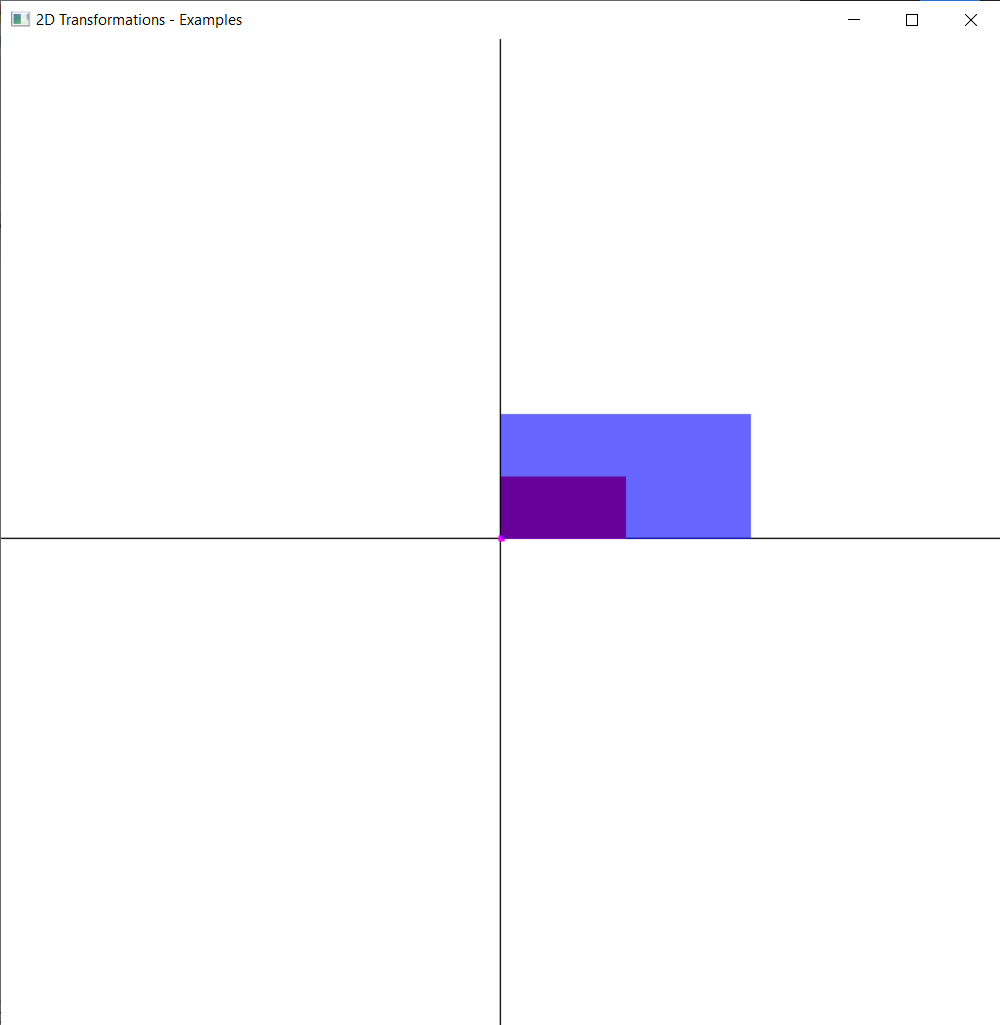
\includegraphics[height=15cm, width=15cm]{Outputs/Output-9.png}
\end{figure}

%Output
\newpage
\subsection*{\flushleft{Output: Console}}
\begin{figure}[h]
\centering
\caption{Console.}
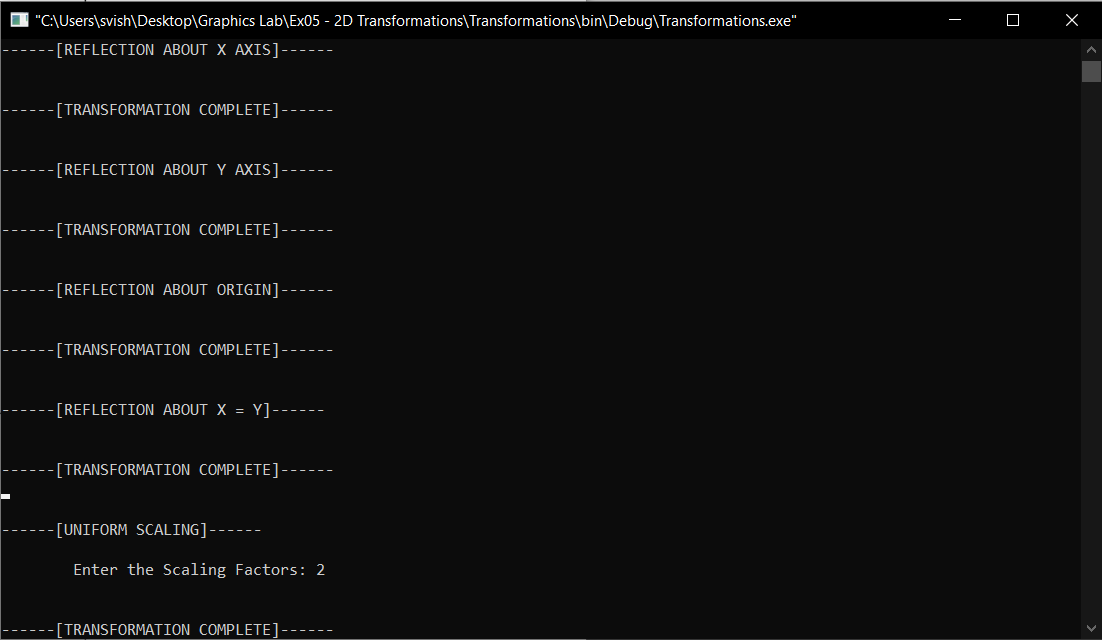
\includegraphics[height=12cm, width=17cm]{Outputs/Console-9.png}
\end{figure}

%Output
\newpage
\subsection*{\flushleft{Output: Differential Scaling}}
\begin{figure}[h]
\centering
\caption{Differential Scaling by a Factor of $(2, 1.5)$.}
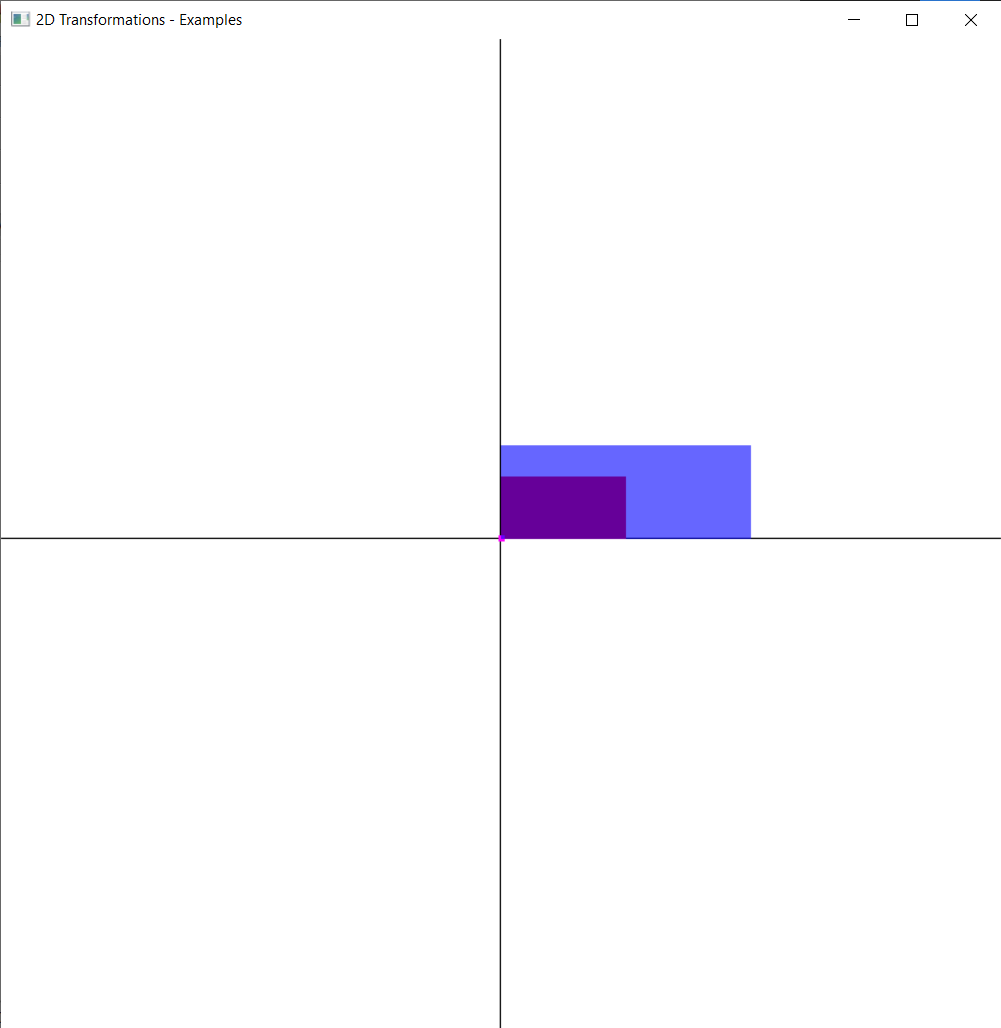
\includegraphics[height=15cm, width=15cm]{Outputs/Output-10.png}
\end{figure}

%Output
\newpage
\subsection*{\flushleft{Output: Differential Scaling About A Fixed Point}}
\begin{figure}[h]
\centering
\caption{Differential Scaling About A Fixed Point $(100, 100)$ by a Factor of $(0.5, 0.75)$.}
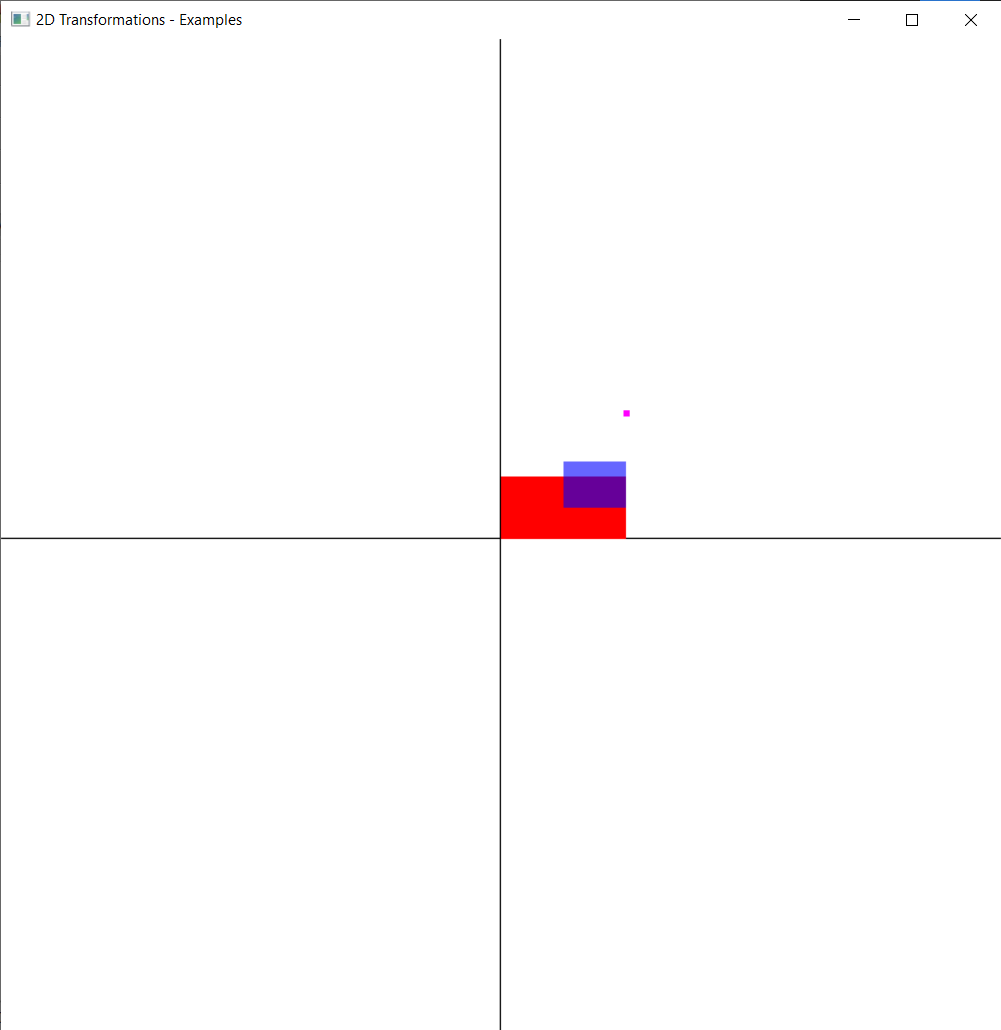
\includegraphics[height=15cm, width=15cm]{Outputs/Output-11.png}
\end{figure}

%Output
\newpage
\subsection*{\flushleft{Output: Console}}
\begin{figure}[h]
\centering
\caption{Console.}
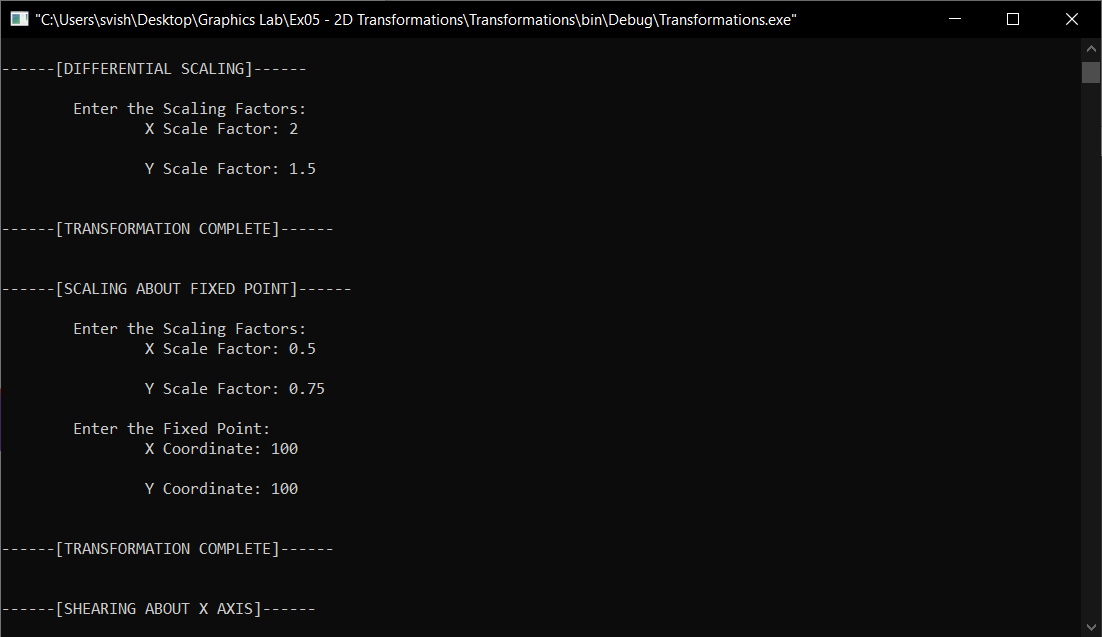
\includegraphics[height=12cm, width=17cm]{Outputs/Console-11.png}
\end{figure}

%Output
\newpage
\subsection*{\flushleft{Output: Shearing About X Axis}}
\begin{figure}[h]
\centering
\caption{Shearing About X Axis by a Parameter of 2.}
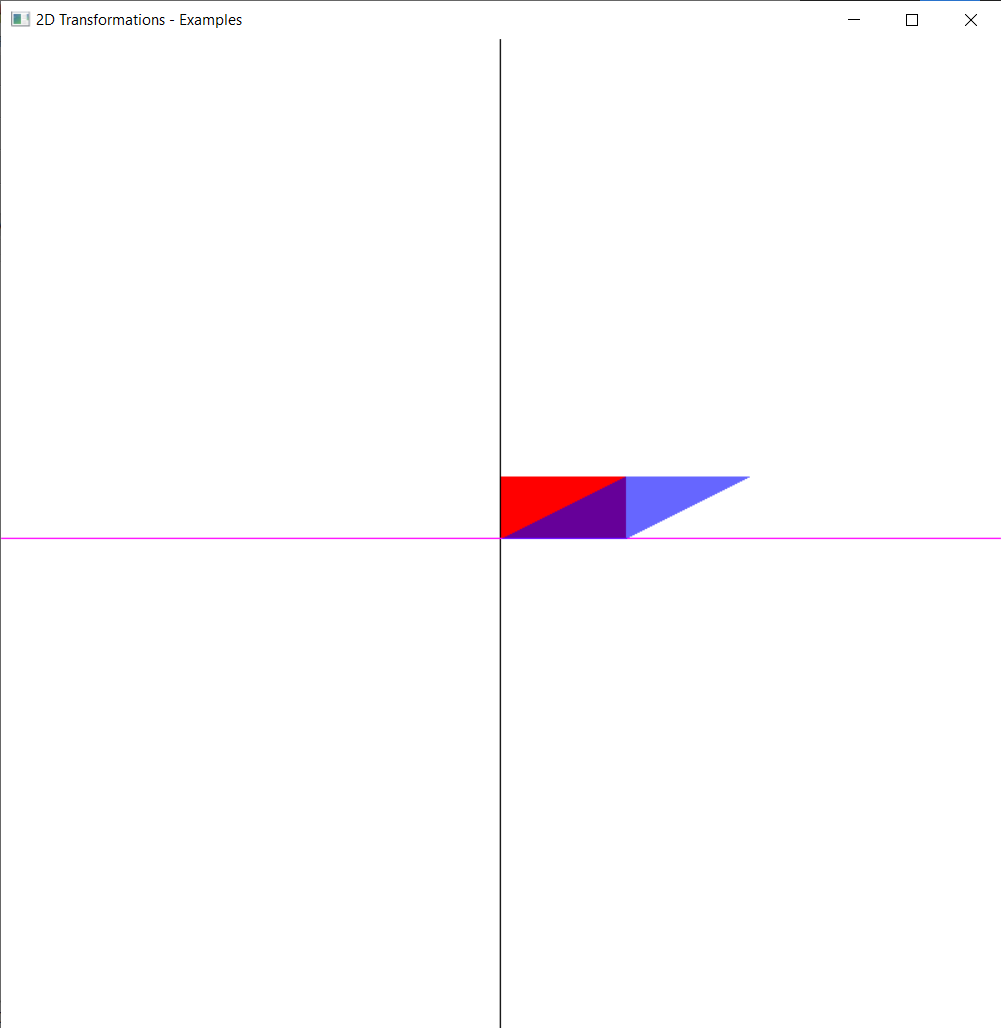
\includegraphics[height=15cm, width=15cm]{Outputs/Output-12.png}
\end{figure}

%Output
\newpage
\subsection*{\flushleft{Output: Shearing About Y Axis}}
\begin{figure}[h]
\centering
\caption{Shearing About Y Axis by a Parameter of 3.}
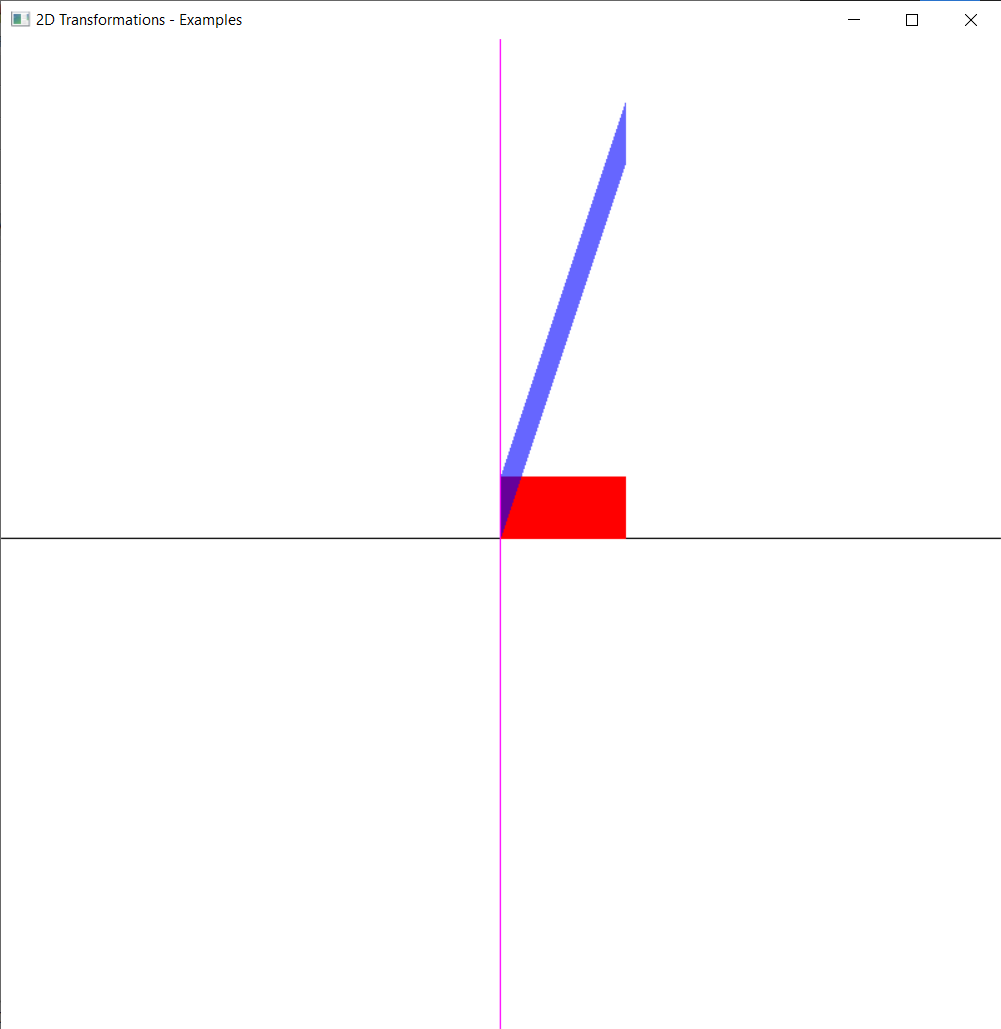
\includegraphics[height=15cm, width=15cm]{Outputs/Output-13.png}
\end{figure}

%Output
\newpage
\subsection*{\flushleft{Output: Shearing About X Axis \& Ref. Line $Y = y$}}
\begin{figure}[h]
\centering
\caption{Shearing About X Axis \& Ref. Line $Y = -100$ by a Parameter of 1.5.}
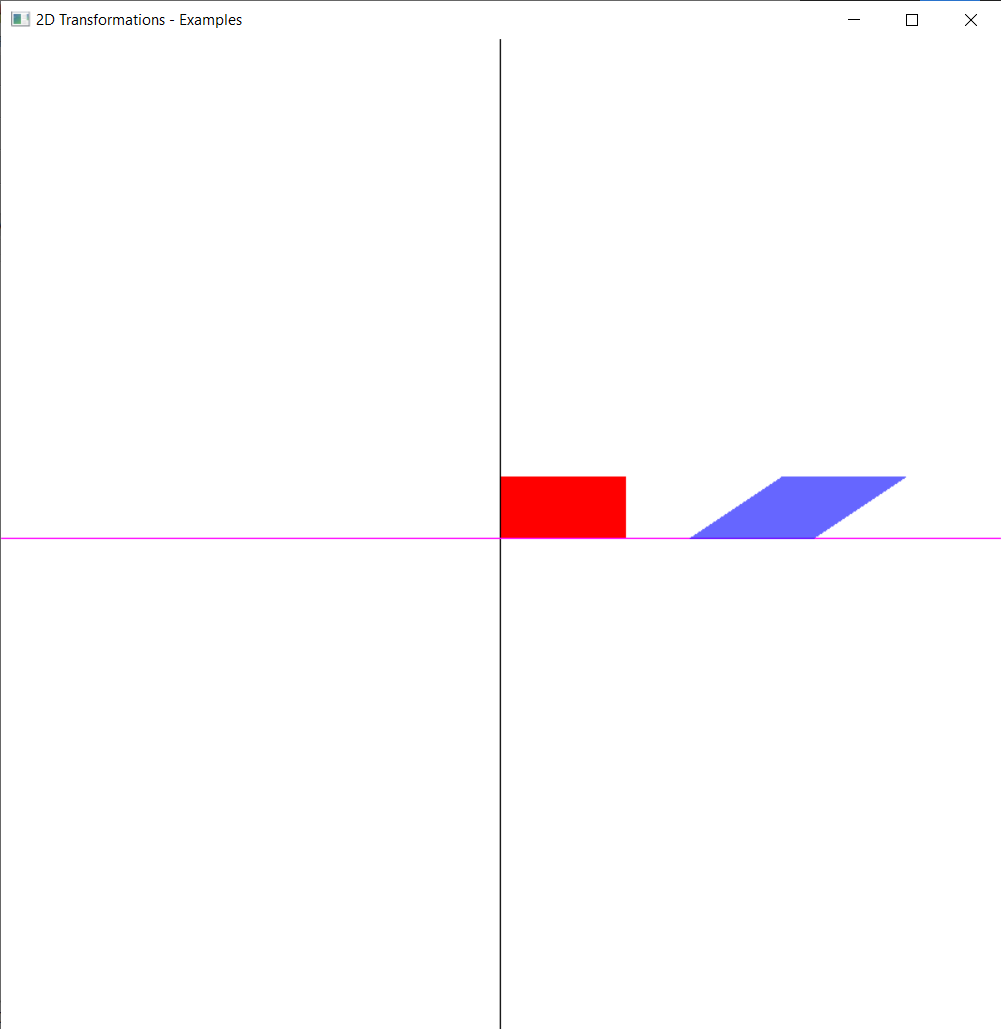
\includegraphics[height=15cm, width=15cm]{Outputs/Output-14.png}
\end{figure}

%Output
\newpage
\subsection*{\flushleft{Output: Shearing About Y Axis \& Ref. Line $X = x$}}
\begin{figure}[h]
\centering
\caption{Shearing About Y Axis \& Ref. Line $X = 100$ by a Parameter of 3.5.}
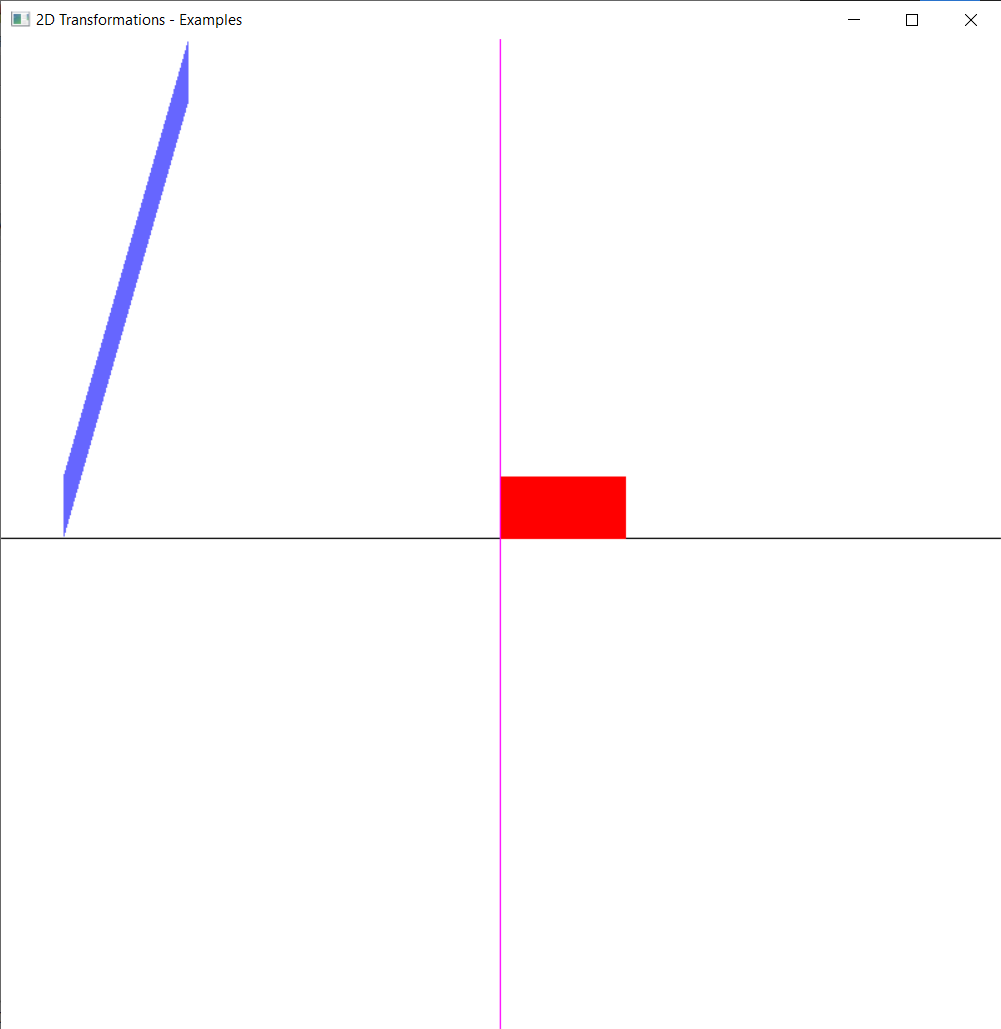
\includegraphics[height=15cm, width=15cm]{Outputs/Output-15.png}
\end{figure}

%Output
\newpage
\subsection*{\flushleft{Output: Console}}
\begin{figure}[h]
\centering
\caption{Console.}
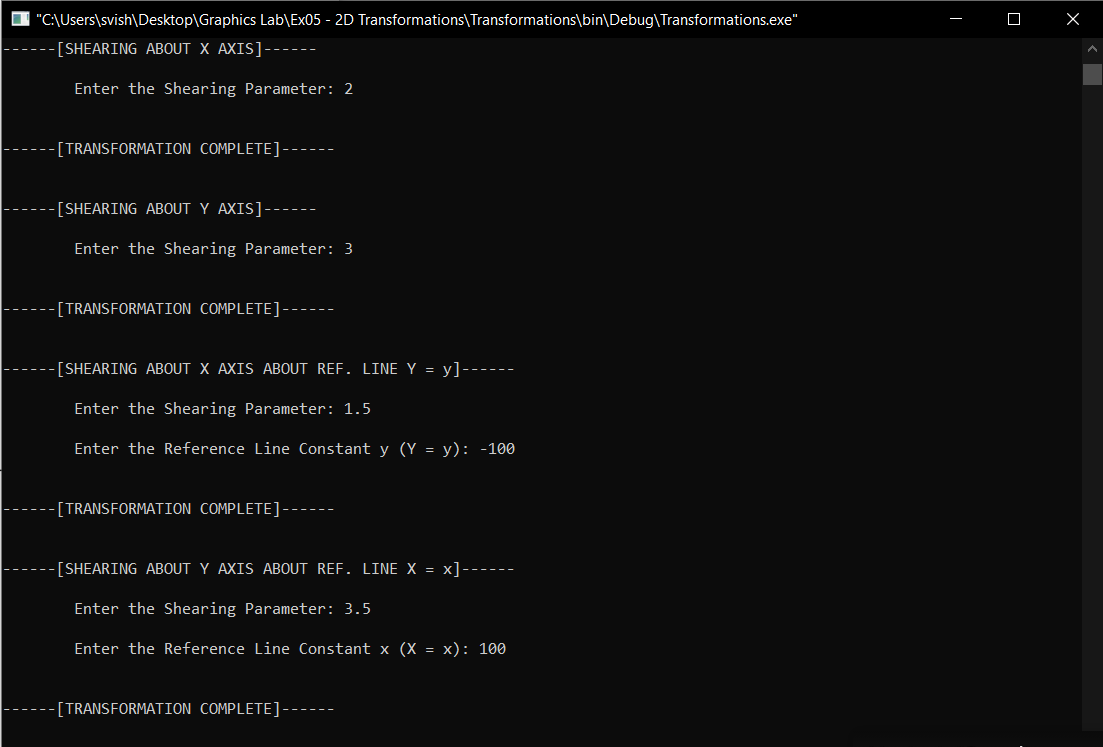
\includegraphics[height=12cm, width=17cm]{Outputs/Console-15.png}
\end{figure}

%Output
\newpage
\subsection*{\flushleft{Output: Changed Base Polygon and its Y Axis Reflection}}
\begin{figure}[h]
\centering
\caption{Changed Base Polygon and its Y Axis Reflection}
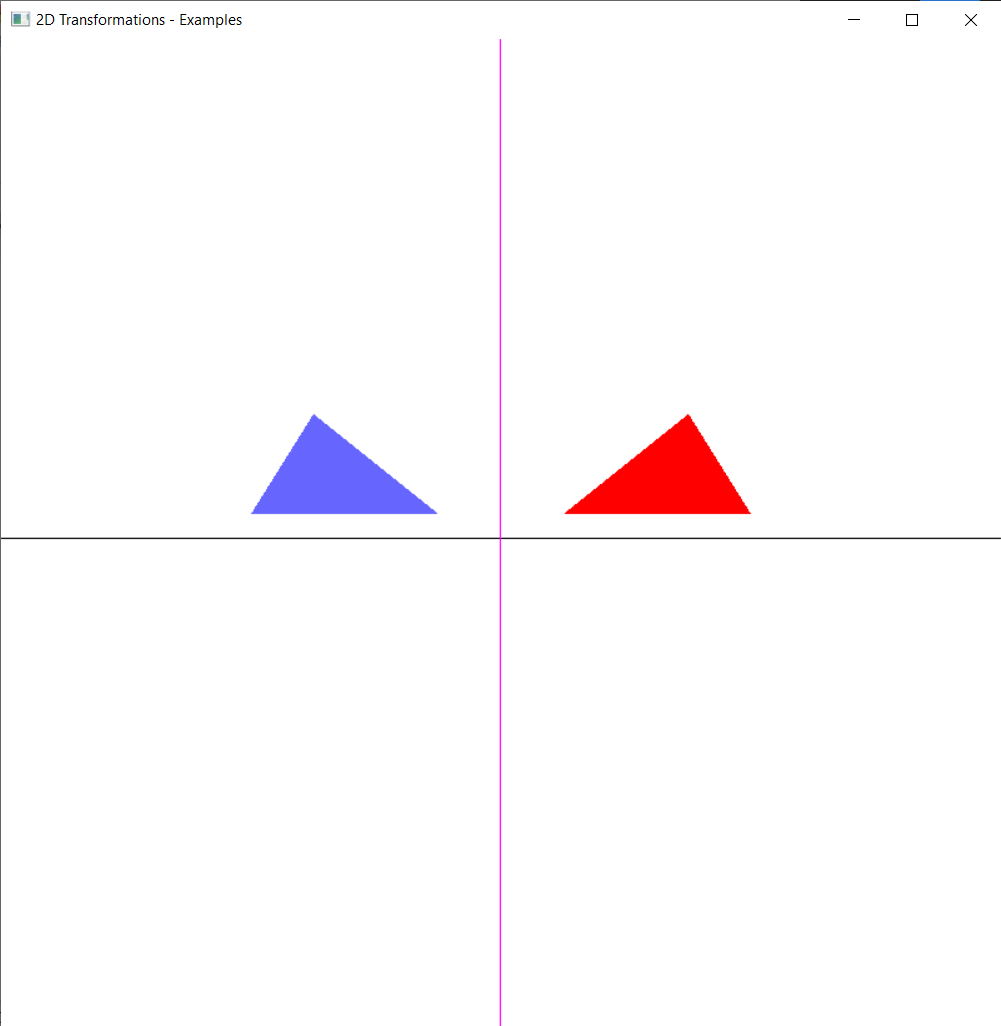
\includegraphics[height=15cm, width=15cm]{Outputs/Output-16.png}
\end{figure}

%Output
\newpage
\subsection*{\flushleft{Output: Console}}
\begin{figure}[h]
\centering
\caption{Console.}
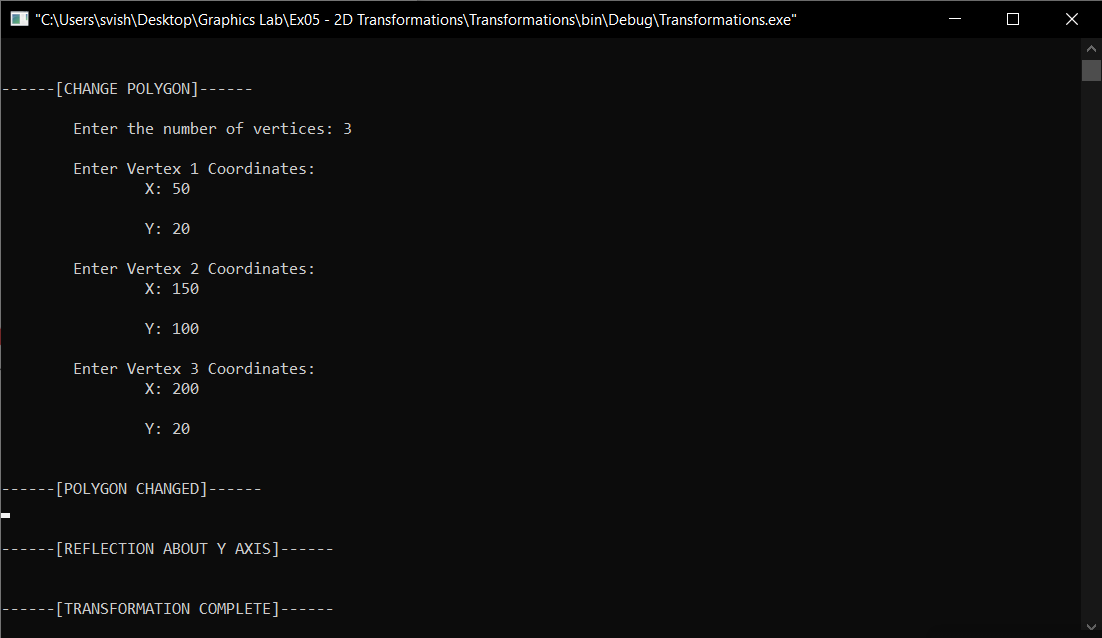
\includegraphics[height=12cm, width=17cm]{Outputs/Console-16.png}
\end{figure}


%Learning Outcome
\newpage
\subsection*{\flushleft{Learning Outcome:}}
\begin{itemize}
\item I understood how to convert $(x, y)$ global coordinates into \textbf{homogeneous coordinates} and its relevance in applying transformations.
\item I understood how to apply \textbf{matrix multiplication} operations to achieve various 2-D Transformations.
\item I learnt about the transformation matrices for translation, rotation, reflection, scaling \& shearing.
\item I implemented separate classes for \textbf{PolygonShape} and \textbf{Point} for ease of use and modularizing the program.
\item I understood how to implement a \textbf{GLUT Menu} for a menu-based approach to apply transformations.
\item I understood how to draw translucent objects with the help of \textbf{glDepthMask(), glBlendFunc() and glColor4f()} with parameter \textbf{ALPHA}.
\item I learnt how to project a \textbf{Cartesian Plane} with the use of \textbf{gluOrtho2D()}.
\item I learnt to use \textbf{enum} to simplify and enhance readability for my menu-driven program.
\item I learnt how to use default arguments in C++ to provide default variables.
\item I implemented \textbf{translation} about a given translation vector.
\item I implemented \textbf{rotation} about an angle $\theta$ and optionally about a pivot point $(x_r, y_r)$.
\item I implemented \textbf{reflection} about X-Axis, Y-Axis, Origin and the line $X = Y$.
\item I implemented \textbf{scaling} uniformly, differentially and optionally about a fixed point $(x_f, y_f)$.
\item I implemented \textbf{shearing} about X-Axis and Y-Axis and optionally to include a reference line $Y = y$ and $X = x$ respectively.
\item I created a function that allows the user to change the base polygon shape outputted in the window.
\item I emphasized the use of \textbf{different colors} to highlight the transformed image, fixed points (if any) and reference lines (if any).
\item I understood that OpenGL code executes in an \textbf{event-driven fashion}, thus while it waits for user-input, the output window might be stalled (unresponsive) and might need to be refreshed after the user I/O has finished.

\end{itemize}


\end{document}